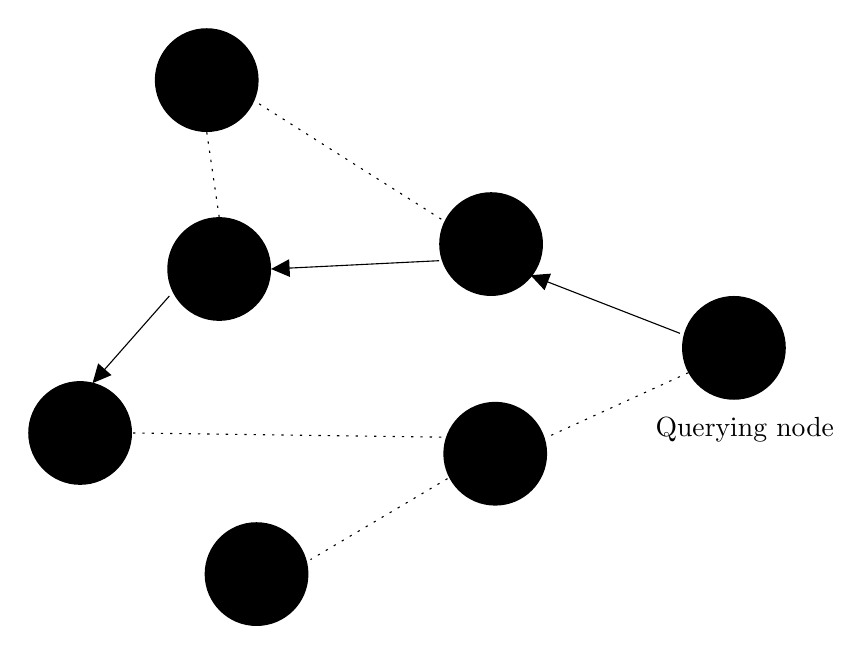
\begin{tikzpicture}[x=0.75pt,y=0.75pt,yscale=-1,xscale=1]
%uncomment if require: \path (0,451); %set diagram left start at 0, and has height of 451

%Shape: Circle [id:dp9331094894799612] 
    \draw  [draw opacity=0][fill={rgb, 255:red, 0; green, 0; blue, 0 }  ,fill opacity=1 ] (119,249) .. controls (119,235.19) and (130.19,224) .. (144,224) .. controls (157.81,224) and (169,235.19) .. (169,249) .. controls (169,262.81) and (157.81,274) .. (144,274) .. controls (130.19,274) and (119,262.81) .. (119,249) -- cycle ;
%Shape: Circle [id:dp9877389362602726] 
    \draw  [draw opacity=0][fill={rgb, 255:red, 0; green, 0; blue, 0 }  ,fill opacity=1 ] (317,158) .. controls (317,144.19) and (328.19,133) .. (342,133) .. controls (355.81,133) and (367,144.19) .. (367,158) .. controls (367,171.81) and (355.81,183) .. (342,183) .. controls (328.19,183) and (317,171.81) .. (317,158) -- cycle ;
%Shape: Circle [id:dp0016664462798891] 
    \draw  [draw opacity=0][fill={rgb, 255:red, 0; green, 0; blue, 0 }  ,fill opacity=1 ] (319,259) .. controls (319,245.19) and (330.19,234) .. (344,234) .. controls (357.81,234) and (369,245.19) .. (369,259) .. controls (369,272.81) and (357.81,284) .. (344,284) .. controls (330.19,284) and (319,272.81) .. (319,259) -- cycle ;
%Shape: Circle [id:dp3393753853906585] 
    \draw  [draw opacity=0][fill={rgb, 255:red, 0; green, 0; blue, 0 }  ,fill opacity=1 ] (180,79) .. controls (180,65.19) and (191.19,54) .. (205,54) .. controls (218.81,54) and (230,65.19) .. (230,79) .. controls (230,92.81) and (218.81,104) .. (205,104) .. controls (191.19,104) and (180,92.81) .. (180,79) -- cycle ;
%Shape: Circle [id:dp6653810548572199] 
    \draw  [draw opacity=0][fill={rgb, 255:red, 0; green, 0; blue, 0 }  ,fill opacity=1 ] (434,208) .. controls (434,194.19) and (445.19,183) .. (459,183) .. controls (472.81,183) and (484,194.19) .. (484,208) .. controls (484,221.81) and (472.81,233) .. (459,233) .. controls (445.19,233) and (434,221.81) .. (434,208) -- cycle ;
%Straight Lines [id:da22721998614149208] 
    \draw    (433,201) -- (363.8,174.09) ;
    \draw [shift={(361,173)}, rotate = 21.25] [fill={rgb, 255:red, 0; green, 0; blue, 0 }  ][line width=0.08]  [draw opacity=0] (8.93,-4.29) -- (0,0) -- (8.93,4.29) -- cycle    ;
%Shape: Circle [id:dp23503433874211244] 
    \draw  [draw opacity=0][fill={rgb, 255:red, 0; green, 0; blue, 0 }  ,fill opacity=1 ] (186,170) .. controls (186,156.19) and (197.19,145) .. (211,145) .. controls (224.81,145) and (236,156.19) .. (236,170) .. controls (236,183.81) and (224.81,195) .. (211,195) .. controls (197.19,195) and (186,183.81) .. (186,170) -- cycle ;
%Straight Lines [id:da49607654384730693] 
    \draw  [dash pattern={on 0.84pt off 2.51pt}]  (318,146) -- (228,89) ;
%Straight Lines [id:da7736178088954417] 
    \draw    (317,166) -- (239,169.85) ;
    \draw [shift={(236,170)}, rotate = 357.17] [fill={rgb, 255:red, 0; green, 0; blue, 0 }  ][line width=0.08]  [draw opacity=0] (8.93,-4.29) -- (0,0) -- (8.93,4.29) -- cycle    ;
%Straight Lines [id:da4613250022232429] 
    \draw    (187,183) -- (151.98,222.75) ;
    \draw [shift={(150,225)}, rotate = 311.38] [fill={rgb, 255:red, 0; green, 0; blue, 0 }  ][line width=0.08]  [draw opacity=0] (8.93,-4.29) -- (0,0) -- (8.93,4.29) -- cycle    ;
%Straight Lines [id:da5738181000901116] 
    \draw  [dash pattern={on 0.84pt off 2.51pt}]  (437,220) -- (369,251) ;
%Shape: Circle [id:dp11048151315696086] 
    \draw  [draw opacity=0][fill={rgb, 255:red, 0; green, 0; blue, 0 }  ,fill opacity=1 ] (204,317) .. controls (204,303.19) and (215.19,292) .. (229,292) .. controls (242.81,292) and (254,303.19) .. (254,317) .. controls (254,330.81) and (242.81,342) .. (229,342) .. controls (215.19,342) and (204,330.81) .. (204,317) -- cycle ;
%Straight Lines [id:da9165977584013065] 
    \draw  [dash pattern={on 0.84pt off 2.51pt}]  (211,145) -- (205,104) ;
%Straight Lines [id:da5283181536620382] 
    \draw  [dash pattern={on 0.84pt off 2.51pt}]  (318,251) -- (169,249) ;
%Straight Lines [id:da7410818285653099] 
    \draw  [dash pattern={on 0.84pt off 2.51pt}]  (321,271) -- (255,310) ;

% Text Node
    \draw (420,240) node [anchor=north west][inner sep=0.75pt]   [align=left] {Querying node};


\end{tikzpicture}
